\documentclass{exam}
\pagestyle{headandfoot}
\firstpageheadrule
\runningheadrule
\firstpageheader{CT}{}{Sam Robbins}
\runningheader{CT}{What is computer software}{Sam Robbins}
\firstpagefooter{}{}{}
\runningfooter{}{}{}

\renewcommand{\solutiontitle}{\noindent\textbf{Solution:}\par\noindent}

\printanswers
\usepackage{graphicx}
\marksnotpoints
\bracketedpoints
\pointsdroppedatright
\pointsinrightmargin
\usepackage{amsmath}
\begin{document}
\begin{center}
	\underline{\huge What is computer software?}
\end{center}
\begin{questions}
\question[5]Briefly (and, necessarily, without being too precise) explain the difference
between an algorithm and a program. Suppose we have an
algorithm and wish to implement it in Python. How many different
implementations are there of this algorithm? 
\begin{solution}[2in]
An algorithm is a sequence of precise instructions that can be applied to specific data items. A program is the implementation of the algorithm in a form that can be executed by a computer, or at least compiled to a form that can be executed by a computer. There are many different implementations of an algorithm as a program.
\end{solution}
\question[6]Give 4 different programming paradigms and briefly explain the underlying
principle for each paradigm.
\begin{solution}[2in]
\textbf{Imperative}: Statements change a programs state (closest to "memory abstraction" of CPU)\\
\textbf{Declarative}: Programs say what to do, rather than how to do it\\
\textbf{Data-Oriented}: Programs work with data through manipulating and searching relations (tables). Tables have things in common that can be linked together to get more information\\
\textbf{Scripting}: Designed to automate frequently used tasks that involve calling or passing commands to external programs. These languages have lots of libraries to make things easier to do
\end{solution}

\question[4]Give 4 different drivers of the evolution of programming languages and
briefly explain each of these driving motivations.
\begin{solution}[2in]
\textbf{Productivity}: Speed up software development process, reduce times and costs, support fast user interface development. This lead to the development of rapid application development (RAD) languages and scripting languages\\
\textbf{Reliability}: To try and reduce the number of errors caused during the execution of the program, this includes things such as type checking and exception handling.\\
\textbf{Security}: Scripting languages used for webpages can, when run on machines, enable malicious programmers to breach your security.\\
\textbf{Execution}: Different programming languages will work better for multi-threading and multi-core processing, allowing parallel computing\\
\end{solution}

\question[3]Give 3 general properties any programming language should have.
\begin{solution}[2in]
\begin{itemize}
	\item Be easy to use, with its programs easy to read, write and understand
	\item Support abstraction so that adding new features and concepts should be possible
	\item Support testing, debugging and program verification
	\item Be inexpensive to use, in terms of execution time, memory usage and maintenance costs
\end{itemize}
\end{solution}

\question[4]Explain very briefly how a Prolog program computes.
\begin{solution}[2in]
A Prolog program consists of a list of facts (atoms) and rules that can be applied to the facts. It then takes queries about the facts which it can answer using the atoms and the rules.
\end{solution}

\question[8]Outline how you would develop a Prolog program that given some facts
about who is the mother or father of whom (in some collection of individuals),
computes who is the grandmother, grandfather or descendant
of whom.
\begin{solution}[2in]
grandma(X,Y) :- mother(X,Z), parents(\_,Z,Y).\\ 
grandma(X,Y) :- mother(X,Z), father(Z,Y).\\ 
grandpa(X,Y) :- father(X,Z), parents(\_,Z,Y). \\
grandpa(X,Y) :- father(X,Z), father(Z,Y). \\
descend(X,Y) :- mother(X,Y)\\
descend(X,Y) :- father(X,Y)\\
descend(X,Y) :- descend(X,Z) , descend(Z,Y)\\
\end{solution}

\question[2]What is the fundamental principle of the research area known as ubiquitous
computing?
\begin{solution}[2in]
The integration of computers and software into everyday objects and activities so that we can control remote aspects of our lives, mostly through RFID.
\end{solution}

\question[2]Give two illustrations of principles of Computational Thinking in the
context of software. 
\begin{solution}[2in]
	Green Computing:An area of computer science involving energy conservation within the world of information technology. This involves writing the main unit of resource is energy expended.\\
	Parallel processing: Certain kinds of problems can be conveniently represented as multiple communicating threads which help to structure code in a more modular manner, e.g., by modelling user interface components as separate threads.
\end{solution}

\question[6]What are the syntax and the semantics of a programming language?
Give 2 reasons why we should strive for a formal semantics for a programming
language.
\begin{solution}[2in]
	\textbf{Syntax}: the rules the govern what makes a program ‘legitimately written’\\
	\textbf{Semantics}: the rules which govern what a program ‘means’\\
	Formal semantics are needed in a programming language so that the programmer is left in no doubt as to what the program will do when it is executed. Without formal semantics we can no longer prove that a program will do what it is intended to do or even runs the same on different machines (with no semantics, processors may interpret the commands differently)
\end{solution}


\question[6]In order to execute a high-level program we must first convert it into machine code so that the CPU can 'understand' it. Briefly explain the difference between compilation and interpretation. How are Java programs executed?
\begin{solution}[2in]
	Compilation is where the entire program is converted into a form that can be executed by the processor before the program is run, whilst interpretation is where the program is converted into an executable form while it is run.\\
	Java, however, is compiled into bytecode before run time, this bytecode is then interpreted at runtime
\end{solution}

\question[2]Give an advantage of compilation over interpretation, and of interpretation over compilation
\begin{solution}[2in]
	Compiled programs have faster execution\\
	Interpretation is faster in a development environment where a program is constantly being changed
\end{solution}


\question[8]Outline a more refined view of (the phases of) compilation
\begin{solution}[2in]
	\begin{itemize}
		\item Lexical Analysis - Converts the program into basic syntactic components and converts it into a token stream
		\item Syntax analysis - Converts the token stream into a parse tree
		\item Translation phase - Converts the parse tree into a linear sequence of intermediate code
		\item Code generation - Converts the intermediate code into assembly and then machine code
	\end{itemize}
\end{solution}

\question[2]In compilation, over 50\% of the time taken can be spent on lexical analysis; that is, character handling. In moving from a program as a string of symbols to a token stream, which algebraic construction is usually used to define tokens?
\begin{solution}[2in]
	Regular Expressions
\end{solution}

\question[14]Define carefully what a regular expression is and explain how a regular expression is used to denote a set of strings
\begin{solution}[2in]
	A regular expression over some alphabet $\Sigma$ is defined as follows:
	\begin{itemize}
		\item Any $a\in \Sigma$ is a regular expression
		\item $\emptyset$ and $\epsilon$ are special regular expressions
		\item If $\omega$ and $\omega'$ are regular expressions, then so are
		\begin{itemize}
			\item $(\omega\omega')$
			\item $(\omega|\omega')$
			\item $(\omega^*)$
		\end{itemize}
	\end{itemize}
	Every regular expression denotes a set of strings over $\Sigma$
	\begin{itemize}
		\item $a,\emptyset$ and $\epsilon$ denote the sets of strings $\{a\},{}$ and $\{\epsilon\}$ respectively
		\item If $\omega$ and $\omega'$ denote the sets of strings R and S then:
		\begin{itemize}
			\item $(\omega\omega')$ denotes \(\{x y : x \in R, y \in S\}\)
			\item $(\omega|\omega')$ denotes $R\cup S$
			\item $(\omega^*)$ denotes \(\left\{x_{1} x_{2} \ldots x_{n} : n \geq 0, x_{1}, x_{2}, \ldots, x_{n} \in R\right\}\)
		\end{itemize}
	\end{itemize}
\end{solution}

\question[5]Give a regular expression that denotes the set of strings over the alphabet $\{a,b,c\}$ consisting of strings with the property that there is always at most one c
\begin{solution}[2in]
	$$((a|b)^*|c)(a|b)^*$$
\end{solution}

\question[7]Give a regular expression that denotes the set of strings over the alphabet $\{a,b\}$ consisting of strings with the property that $a$ must always be followed by $bb$
\begin{solution}[2in]
	$(b|abb)^*$
\end{solution}

\question[8]Define carefully a finite state machine and explain how one is used to accept a set of strings
\begin{solution}[2in]
	A finite state machine is defined as:
	\[
	M=\left(\Sigma, Q, \delta : Q \times \Sigma \rightarrow Q, q_{0} \in Q, F\right)
	\]
	where
	\begin{itemize}
		\item $\Sigma$ is some finite alphabet
		\item $Q$ is some finite set of states with initial state $q_0$ and set of final states $F\subseteq Q$
		\item $\delta: Q\times \Sigma \rightarrow Q$ is the transition function
	\end{itemize}
On input any string $a_1a_2...a_n$ over $\Sigma$ (where $n \geq 0$, and so we may input the empty string if we wish), M yields a sequence of states $q_0,q_1,q_2,...,q_n$ via:
\[
q_{1}=\delta\left(q_{0}, a_{1}\right), q_{2}=\delta\left(q_{1}, a_{2}\right), q_{3}=\delta\left(q_{2}, a_{3}\right), \ldots, q_{n}=\delta\left(q_{n-1}, a_{n}\right)
\]
The input string is accepted by our FSM M if the resulting sequence of states $q_0,q_1,q_2,...,q_n$ ends in a final state; that is, is such that $q_n\in F$. This M accepts a set of strings over $\Sigma$
\end{solution}


\question[5]Give a finite state machine that accepts the set of strings over the alphabet $\{a,b,c\}$ consisting of strings with the property that there is always at most one c
\begin{solution}[2in]
	\begin{center}
		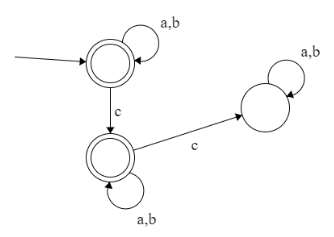
\includegraphics[scale=0.7]{Q18}
	\end{center}	
\end{solution}


\question[7]Give a finite state machine that accepts the set of strings over the alphabet $\{a,b\}$ consisting of strings with the property that any a bust always be followed by bb
\begin{solution}[2in]
	\begin{center}
		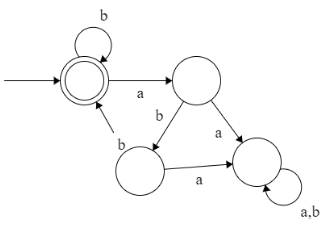
\includegraphics[scale=0.7]{Q19}
	\end{center}
	
\end{solution}

\question[2]What is the relationship between regular expressions and finite state machines?
\begin{solution}[2in]
	A set of strings is represented by a regular expression iff it is accepted by a FSM
\end{solution}

\question[10]Define carefully a context-free grammar and explain how one is used to generate a set of string
\begin{solution}[2in]
	A grammar is a tuple $(N,T,s,R)$ where
	\begin{itemize}
		\item T and N are disjoint finite sets of terminal and non-terminal symbols, respectively
		\item $s\in N$ is the start symbol
		\item R is a finite set of productions or rules so that
		\[
		R \subseteq(N \cup T)^{+} \times(N \cup T)^{*}
		\]
		and where if $(\alpha,\beta)\in R$ when $\alpha$ contains at least one symbol\\
	\end{itemize}
		In a context free grammar productions are of the form
		\[
		b \rightarrow a_{1} a_{2} \ldots a_{k}, \text { with } k>0, b \in N, \text { and } a_{1}, a_{2}, \ldots, a_{k} \in N \cup T
		\]
	A production $b\rightarrow a_1a_2...a_k$ can be applied to a string $\omega$ containg b via:
	\[
	\omega=\ldots b^{\prime} \underline{b} b^{\prime} \cdots \Rightarrow \omega^{\prime}=\ldots b^{\prime} a_{1} a_{2} \dots a_{k} b^{\prime} \ldots
	\]
	
\end{solution}

\question[5]What restriction on context-free grammar makes it a regular grammar, and how are regular grammars, regular expressions and finite state machines related?
\begin{solution}[2in]
	Regular grammar (N,T,s,R) is a context free grammar where all productions are one of the following orms:
	\begin{itemize}
		\item $b\rightarrow a$ where $a\in T$
		\item $b\rightarrow ac$ where $a\in T$ and $c\in N$
		\item $b\rightarrow \epsilon$
	\end{itemize}
	
	A regular expression can always be written in a context free grammar, but not all context-free grammars can be expressed by a regular expression or FSM. A regular grammar can always be written as a regular expression or FSM
\end{solution}


\question[5]Define a regular grammar that generates the set of strings over the alphabet $\{a,b,c\}$ consisting of strings with the property that there is always at most one c
\begin{solution}[2in]
	$$(N=\{s,t\},T=\{a,b,c\},s,R)$$
	Where R is:
	$$s\rightarrow \epsilon \quad s\rightarrow as \quad s\rightarrow bs \quad t\rightarrow cs \quad t \rightarrow au \quad t\rightarrow bu \quad t\rightarrow \epsilon$$
\end{solution}


\question[7]Define a regular grammar that generates the set of strings over the alphabet $\{a,b\}$ consisting of strings with the property that any a must always be followed by $bb$
\begin{solution}[2in]
	$$(N=\{s,t,u,v\},T=\{a,b\},s,R)$$
	Where R is
	$$s\rightarrow \epsilon \quad u\rightarrow as \quad s \rightarrow bs \quad v\rightarrow bu \quad t\rightarrow bv \quad t\rightarrow bt \quad t\rightarrow \epsilon \quad u\rightarrow at$$
\end{solution}

\question[1]Which algebraic notation is normally used to specify the syntax of a programming language
\begin{solution}[2in]
	Bakus Naur Form
\end{solution}


\end{questions}



\end{document}